
\documentclass[letterpaper,hide notes,xcolor={table,svgnames},pdftex,10pt]{beamer}
\def\showexamples{t}


%\usepackage[svgnames]{xcolor}

%% Demo talk
%\documentclass[letterpaper,notes=show]{beamer}

\usecolortheme{crane}
\setbeamertemplate{navigation symbols}{}

\usetheme{MyPittsburgh}
%\usetheme{Frankfurt}

%\usepackage{tipa}

\usepackage{hyperref}
\usepackage{graphicx,xspace}
\usepackage[normalem]{ulem}
\usepackage{multicol}
\usepackage{amsmath,amssymb,amsthm,graphicx,xspace}
\newcommand\SF[1]{$\bigstar$\footnote{SF: #1}}

\usepackage[default]{sourcesanspro}
\usepackage[T1]{fontenc}
\usepackage[scaled]{beramono}
\usepackage{tikzpagenodes}

\newcounter{tmpnumSlide}
\newcounter{tmpnumNote}


% old question code
%\newcommand\question[1]{{$\bigstar$ \small \onlySlide{2}{#1}}}
% \newcommand\nquestion[1]{\ifdefined \presentationonly \textcircled{?} \fi \note{\par{\Large \textbf{?}} #1}}
% \newcommand\nanswer[1]{\note{\par{\Large \textbf{A}} #1}}


 \newcommand\mnote[1]{%
   \addtocounter{tmpnumSlide}{1}
   \ifdefined\showcues {~\tiny\fbox{\arabic{tmpnumSlide}}}\fi
   \note{\setlength{\parskip}{1ex}\addtocounter{tmpnumNote}{1}\textbf{\Large \arabic{tmpnumNote}:} {#1\par}}}

\newcommand\mmnote[1]{\note{\setlength{\parskip}{1ex}#1\par}}

%\newcommand\mnote[2][]{\ifdefined\handoutwithnotes {~\tiny\fbox{#1}}\fi
% \note{\setlength{\parskip}{1ex}\textbf{\Large #1:} #2\par}}

%\newcommand\mnote[2][]{{\tiny\fbox{#1}} \note{\setlength{\parskip}{1ex}\textbf{\Large #1:} #2\par}}

\newcommand\mquestion[2]{{~\color{red}\fbox{?}}\note{\setlength{\parskip}{1ex}\par{\Large \textbf{?}} #1} \note{\setlength{\parskip}{1ex}\par{\Large \textbf{A}} #2\par}\ifdefined \presentationonly \pause \fi}

\newcommand\blackboard[1]{%
\ifdefined   \showblackboard
  {#1}
  \else {\begin{center} \fbox{\colorbox{blue!30}{%
         \begin{minipage}{.95\linewidth}%
           \hspace{\stretch{1}} Some space intentionally left blank; done at the blackboard.%
         \end{minipage}}}\end{center}}%
         \fi%
}



%\newcommand\q{\tikz \node[thick,color=black,shape=circle]{?};}
%\newcommand\q{\ifdefined \presentationonly \textcircled{?} \fi}

\usepackage{listings}
\lstset{basicstyle=\footnotesize\ttfamily,
	breaklines=true,
	aboveskip=15pt,
  	belowskip=15pt,
	frame=lines,
	numbers=left, basicstyle=\scriptsize, numberstyle=\tiny, stepnumber=0, numbersep=2pt
}

\usepackage{siunitx}
\newcommand\sius[1]{\num[group-separator = {,}]{#1}\si{\micro\second}}
\newcommand\sims[1]{\num[group-separator = {,}]{#1}\si{\milli\second}}
\newcommand\sins[1]{\num[group-separator = {,}]{#1}\si{\nano\second}}
\sisetup{group-separator = {,}, group-digits = true}

%% -------------------- tikz --------------------
\usepackage{tikz}
\usetikzlibrary{positioning}
\usetikzlibrary{arrows,backgrounds,automata,decorations.shapes,decorations.pathmorphing,decorations.markings,decorations.text,decorations.pathreplacing}

\tikzstyle{place}=[circle,draw=blue!50,fill=blue!20,thick, inner sep=0pt,minimum size=6mm]
\tikzstyle{transition}=[rectangle,draw=black!50,fill=black!20,thick, inner sep=0pt,minimum size=4mm]

\tikzstyle{block}=[rectangle,draw=black, thick, inner sep=5pt]
\tikzstyle{bullet}=[circle,draw=black, fill=black, thin, inner sep=2pt]

\tikzstyle{pre}=[<-,shorten <=1pt,>=stealth',semithick]
\tikzstyle{post}=[->,shorten >=1pt,>=stealth',semithick]
\tikzstyle{bi}=[<->,shorten >=1pt,shorten <=1pt, >=stealth',semithick]

\tikzstyle{mut}=[-,>=stealth',semithick]

\tikzstyle{treereset}=[dashed,->, shorten >=1pt,>=stealth',thin]

\usepackage{ifmtarg}
\usepackage{xifthen}
\makeatletter
% new counter to now which frame it is within the sequence
\newcounter{multiframecounter}
% initialize buffer for previously used frame title
\gdef\lastframetitle{\textit{undefined}}
% new environment for a multi-frame
\newenvironment{multiframe}[1][]{%
\ifthenelse{\isempty{#1}}{%
% if no frame title was set via optional parameter,
% only increase sequence counter by 1
\addtocounter{multiframecounter}{1}%
}{%
% new frame title has been provided, thus
% reset sequence counter to 1 and buffer frame title for later use
\setcounter{multiframecounter}{1}%
\gdef\lastframetitle{#1}%
}%
% start conventional frame environment and
% automatically set frame title followed by sequence counter
\begin{frame}%
\frametitle{\lastframetitle~{\normalfont(\arabic{multiframecounter})}}%
}{%
\end{frame}%
}
\makeatother

\makeatletter
\newdimen\tu@tmpa%
\newdimen\ydiffl%
\newdimen\xdiffl%
\newcommand\ydiff[2]{%
    \coordinate (tmpnamea) at (#1);%
    \coordinate (tmpnameb) at (#2);%
    \pgfextracty{\tu@tmpa}{\pgfpointanchor{tmpnamea}{center}}%
    \pgfextracty{\ydiffl}{\pgfpointanchor{tmpnameb}{center}}%
    \advance\ydiffl by -\tu@tmpa%
}
\newcommand\xdiff[2]{%
    \coordinate (tmpnamea) at (#1);%
    \coordinate (tmpnameb) at (#2);%
    \pgfextractx{\tu@tmpa}{\pgfpointanchor{tmpnamea}{center}}%
    \pgfextractx{\xdiffl}{\pgfpointanchor{tmpnameb}{center}}%
    \advance\xdiffl by -\tu@tmpa%
}
\makeatother
\newcommand{\copyrightbox}[3][r]{%
\begin{tikzpicture}%
\node[inner sep=0pt,minimum size=2em](ciimage){#2};
\usefont{OT1}{phv}{n}{n}\fontsize{4}{4}\selectfont
\ydiff{ciimage.south}{ciimage.north}
\xdiff{ciimage.west}{ciimage.east}
\ifthenelse{\equal{#1}{r}}{%
\node[inner sep=0pt,right=1ex of ciimage.south east,anchor=north west,rotate=90]%
{\raggedleft\color{black!50}\parbox{\the\ydiffl}{\raggedright{}#3}};%
}{%
\ifthenelse{\equal{#1}{l}}{%
\node[inner sep=0pt,right=1ex of ciimage.south west,anchor=south west,rotate=90]%
{\raggedleft\color{black!50}\parbox{\the\ydiffl}{\raggedright{}#3}};%
}{%
\node[inner sep=0pt,below=1ex of ciimage.south west,anchor=north west]%
{\raggedleft\color{black!50}\parbox{\the\xdiffl}{\raggedright{}#3}};%
}
}
\end{tikzpicture}
}


%% --------------------

%\usepackage[excludeor]{everyhook}
%\PushPreHook{par}{\setbox0=\lastbox\llap{MUH}}\box0}

%\vspace*{\stretch{1}

%\setbox0=\lastbox \llap{\textbullet\enskip}\box0}

\setlength{\parskip}{\fill}

\newcommand\noskips{\setlength{\parskip}{1ex}}
\newcommand\doskips{\setlength{\parskip}{\fill}}

\newcommand\xx{\par\vspace*{\stretch{1}}\par}
\newcommand\xxs{\par\vspace*{2ex}\par}
\newcommand\tuple[1]{\langle #1 \rangle}
\newcommand\code[1]{{\sf \footnotesize #1}}
\newcommand\ex[1]{\uline{Example:} \ifdefined \presentationonly \pause \fi
  \ifdefined\showexamples#1\xspace\else{\uline{\hspace*{2cm}}}\fi}

\newcommand\ceil[1]{\lceil #1 \rceil}


\AtBeginSection[]
{
   \begin{frame}
       \frametitle{Outline}
       \tableofcontents[currentsection]
   \end{frame}
}



\pgfdeclarelayer{edgelayer}
\pgfdeclarelayer{nodelayer}
\pgfsetlayers{edgelayer,nodelayer,main}

\tikzstyle{none}=[inner sep=0pt]
\tikzstyle{rn}=[circle,fill=Red,draw=Black,line width=0.8 pt]
\tikzstyle{gn}=[circle,fill=Lime,draw=Black,line width=0.8 pt]
\tikzstyle{yn}=[circle,fill=Yellow,draw=Black,line width=0.8 pt]
\tikzstyle{empty}=[circle,fill=White,draw=Black]
\tikzstyle{bw} = [rectangle, draw, fill=blue!20, 
    text width=4em, text centered, rounded corners, minimum height=2em]
    
    \newcommand{\CcNote}[1]{% longname
	This work is licensed under the \textit{Creative Commons #1 3.0 License}.%
}
\newcommand{\CcImageBy}[1]{%
	\includegraphics[scale=#1]{creative_commons/cc_by_30.pdf}%
}
\newcommand{\CcImageSa}[1]{%
	\includegraphics[scale=#1]{creative_commons/cc_sa_30.pdf}%
}
\newcommand{\CcImageNc}[1]{%
	\includegraphics[scale=#1]{creative_commons/cc_nc_30.pdf}%
}
\newcommand{\CcGroupBySa}[2]{% zoom, gap
	\CcImageBy{#1}\hspace*{#2}\CcImageNc{#1}\hspace*{#2}\CcImageSa{#1}%
}
\newcommand{\CcLongnameByNcSa}{Attribution-NonCommercial-ShareAlike}

\newenvironment{changemargin}[1]{% 
  \begin{list}{}{% 
    \setlength{\topsep}{0pt}% 
    \setlength{\leftmargin}{#1}% 
    \setlength{\rightmargin}{1em}
    \setlength{\listparindent}{\parindent}% 
    \setlength{\itemindent}{\parindent}% 
    \setlength{\parsep}{\parskip}% 
  }% 
  \item[]}{\end{list}} 




\title{Lecture 27 --- Liar, Liar }

\author{Patrick Lam \& Jeff Zarnett \\ \small \texttt{patrick.lam@uwaterloo.ca jzarnett@uwaterloo.ca}}
\institute{Department of Electrical and Computer Engineering \\
  University of Waterloo}
\date{\today}


\begin{document}

\begin{frame}
  \titlepage

 \end{frame}



\begin{frame}
\frametitle{Liar, Liar}

\begin{center}
	
\includegraphics[width=0.75\textwidth]{images/Liar-Liar.jpg}
\end{center}


\end{frame}

\begin{frame}
\frametitle{Sampling Based Profiling}

Let's open with a video that illustrates one of the problems with sampling-based profiling:

\begin{center}
	\url{https://www.youtube.com/watch?v=jQDjJRYmeWg}
\end{center}

Is this fake?

\end{frame}

\part{Lies about Calling Context}

%%%%%%%%%%%%%%%%%%%%%%%%%%%%%%%%%%%%%%%%%%%%%%%%%%%%%%%%%%%%%%%%%%%%%%%%%%%%%%%%
\begin{frame}
  \partpage
\end{frame}
%%%%%%%%%%%%%%%%%%%%%%%%%%%%%%%%%%%%%%%%%%%%%%%%%%%%%%%%%%%%%%%%%%%%%%%%%%%%%%%%

%%%%%%%%%%%%%%%%%%%%%%%%%%%%%%%%%%%%%%%%%%%%%%%%%%%%%%%%%%%%%%%%%%%%%%%%%%%%%%%%
\begin{frame}
  \frametitle{gprof and KCacheGrind}
  
  
    Who can we trust?\\[1em]

    Some profiler results are real. \\
    Other results are interpolated, and perhaps wrong.
    
    \begin{center}
	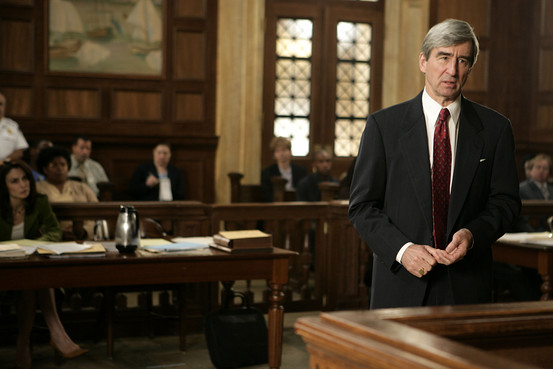
\includegraphics[width=0.6\textwidth]{images/lawandorder.jpg}
	\end{center}
  

  \begin{center}
    Reference: Yossi Kreinin,\\
  \tiny
  \url{http://www.yosefk.com/blog/how-profilers-lie-the-cases-of-gprof-and-kcachegrind.html}
  \end{center}

\end{frame}
%%%%%%%%%%%%%%%%%%%%%%%%%%%%%%%%%%%%%%%%%%%%%%%%%%%%%%%%%%%%%%%%%%%%%%%%%%%%%%%%

%%%%%%%%%%%%%%%%%%%%%%%%%%%%%%%%%%%%%%%%%%%%%%%%%%%%%%%%%%%%%%%%%%%%%%%%%%%%%%%%
\begin{frame}[fragile]
  \frametitle{Running Example}

  \begin{center}
  \begin{minipage}{.7\textwidth}
\begin{lstlisting}
void work(int n) {
  volatile int i=0; //don't optimize away
  while(i++ < n);
}
void easy() { work(1000); }
void hard() { work(1000*1000*1000); }
int main() { easy(); hard(); }
\end{lstlisting}
  \end{minipage}
  \end{center}
  
\end{frame}
%%%%%%%%%%%%%%%%%%%%%%%%%%%%%%%%%%%%%%%%%%%%%%%%%%%%%%%%%%%%%%%%%%%%%%%%%%%%%%%%

%%%%%%%%%%%%%%%%%%%%%%%%%%%%%%%%%%%%%%%%%%%%%%%%%%%%%%%%%%%%%%%%%%%%%%%%%%%%%%%%
\begin{frame}[fragile]
  \frametitle{Running the Running Example}

{\scriptsize
\begin{verbatim}
[plam@lynch L27]$ gprof ./try gmon.out
Flat profile:

Each sample counts as 0.01 seconds.
  %   cumulative   self              self     total           
 time   seconds   seconds    calls  ms/call  ms/call  name    
101.30      1.68     1.68        2   840.78   840.78  work
  0.00      1.68     0.00        1     0.00   840.78  easy
  0.00      1.68     0.00        1     0.00   840.78  hard
\end{verbatim}
}

  That's not right! \\
  {\tt easy} takes $\approx$ 0s, {\tt hard} takes 1.68s.

\end{frame}
%%%%%%%%%%%%%%%%%%%%%%%%%%%%%%%%%%%%%%%%%%%%%%%%%%%%%%%%%%%%%%%%%%%%%%%%%%%%%%%%

%%%%%%%%%%%%%%%%%%%%%%%%%%%%%%%%%%%%%%%%%%%%%%%%%%%%%%%%%%%%%%%%%%%%%%%%%%%%%%%%
\begin{frame}[fragile]
  \frametitle{What's Wrong?}

  
    Need to understand how {\tt gprof} works.\\[1em]
    \begin{itemize}
    \item
      \begin{tabbing}
      {\bf profil()}: \= asks glibc to record which instruction \\
      \> is currently executing
      (100$\times$/second).
      \end{tabbing}
    \item
      \begin{tabbing}
        {\bf mcount()}: \= records call graph edges;\\
        \> called by {\tt -pg} instrumentation.
      \end{tabbing}
    \end{itemize}
~\\
    {\bf profil} information is statistical; \\
    {\bf mcount} information is exact.

\end{frame}
%%%%%%%%%%%%%%%%%%%%%%%%%%%%%%%%%%%%%%%%%%%%%%%%%%%%%%%%%%%%%%%%%%%%%%%%%%%%%%%%

%%%%%%%%%%%%%%%%%%%%%%%%%%%%%%%%%%%%%%%%%%%%%%%%%%%%%%%%%%%%%%%%%%%%%%%%%%%%%%%%
\begin{frame}[fragile]
  \frametitle{Those Numbers Again}

{\scriptsize
\begin{verbatim}
[plam@lynch L27]$ gprof ./try gmon.out
Flat profile:

Each sample counts as 0.01 seconds.
  %   cumulative   self              self     total           
 time   seconds   seconds    calls  ms/call  ms/call  name    
101.30      1.68     1.68        2   840.78   840.78  work
  0.00      1.68     0.00        1     0.00  *840.78* easy
  0.00      1.68     0.00        1     0.00  *840.78* hard
\end{verbatim}
}


  \begin{itemize}
  \item calls: reliable;
  \item self seconds: sampled, but OK here;
    \item total ms/call: interpolated!
  \end{itemize}

\end{frame}
%%%%%%%%%%%%%%%%%%%%%%%%%%%%%%%%%%%%%%%%%%%%%%%%%%%%%%%%%%%%%%%%%%%%%%%%%%%%%%%%

%%%%%%%%%%%%%%%%%%%%%%%%%%%%%%%%%%%%%%%%%%%%%%%%%%%%%%%%%%%%%%%%%%%%%%%%%%%%%%%%
\begin{frame}
  \frametitle{total ms/call}

  gprof sees:
  \begin{itemize}
    \item total of 1.68s in {\tt work},\\
    \item 1 call to {\tt work} from {\tt easy};
    \item 1 call to {\tt work} from {\tt hard}.
  \end{itemize}
  All of these numbers are reliable.\\[1em]
  gprof's unreliable conclusion: \\ {\tt easy}, {\tt hard} 
  both cause 840ms of {\tt work} time.\\[1em]
  
  \alert{Wrong}: {\tt work} takes 1000000$\times$ longer when called from {\tt hard}!

\end{frame}
%%%%%%%%%%%%%%%%%%%%%%%%%%%%%%%%%%%%%%%%%%%%%%%%%%%%%%%%%%%%%%%%%%%%%%%%%%%%%%%%

%%%%%%%%%%%%%%%%%%%%%%%%%%%%%%%%%%%%%%%%%%%%%%%%%%%%%%%%%%%%%%%%%%%%%%%%%%%%%%%%
\begin{frame}
  \frametitle{Where gprof guesses: Call graph edges}
  
    \begin{itemize}
  \item contribution of children to parents;
  \item total runtime spent in self+children;
  \item etc.
    \end{itemize}
  
\end{frame}
%%%%%%%%%%%%%%%%%%%%%%%%%%%%%%%%%%%%%%%%%%%%%%%%%%%%%%%%%%%%%%%%%%%%%%%%%%%%%%%%

%%%%%%%%%%%%%%%%%%%%%%%%%%%%%%%%%%%%%%%%%%%%%%%%%%%%%%%%%%%%%%%%%%%%%%%%%%%%%%%%
\begin{frame}
  \frametitle{When are call graph edges right?}

    Two cases:
    \begin{itemize}
    \item functions with only one caller\\
      (e.g. {\tt f()} only called by {\tt g()}); or,
    \item functions which always take the same time to complete\\
      (e.g. {\tt rand()}).
    \end{itemize}
    ~\\
    What's sketchy:\\
    Any function whose running time depends on its inputs,\\
    and which is called from multiple contexts.
    
  
\end{frame}
%%%%%%%%%%%%%%%%%%%%%%%%%%%%%%%%%%%%%%%%%%%%%%%%%%%%%%%%%%%%%%%%%%%%%%%%%%%%%%%%

%%%%%%%%%%%%%%%%%%%%%%%%%%%%%%%%%%%%%%%%%%%%%%%%%%%%%%%%%%%%%%%%%%%%%%%%%%%%%%%%
\begin{frame}
  \frametitle{KCacheGrind}
  
    KCacheGrind is a frontend to callgrind.\\[1em]
    callgrind is part of valgrind,\\
    and runs the program under an x86 JIT.
  
\end{frame}
%%%%%%%%%%%%%%%%%%%%%%%%%%%%%%%%%%%%%%%%%%%%%%%%%%%%%%%%%%%%%%%%%%%%%%%%%%%%%%%%

%%%%%%%%%%%%%%%%%%%%%%%%%%%%%%%%%%%%%%%%%%%%%%%%%%%%%%%%%%%%%%%%%%%%%%%%%%%%%%%%
\begin{frame}
  \frametitle{KCacheGrind example}
  \begin{center}
    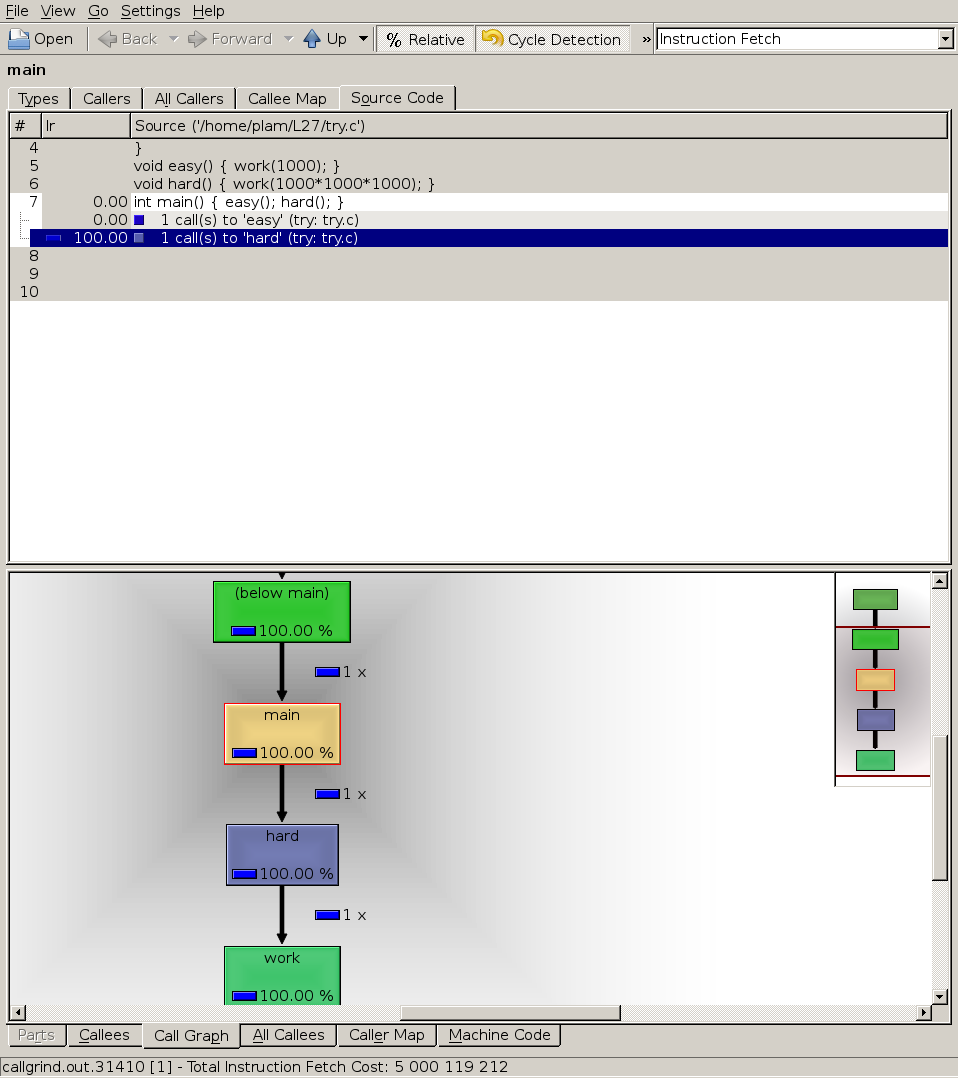
\includegraphics[width=.5\textwidth]{images/kcachegrind}
  \end{center}
  
    Yes, {\tt hard} takes all the time.
  
\end{frame}
%%%%%%%%%%%%%%%%%%%%%%%%%%%%%%%%%%%%%%%%%%%%%%%%%%%%%%%%%%%%%%%%%%%%%%%%%%%%%%%%

%%%%%%%%%%%%%%%%%%%%%%%%%%%%%%%%%%%%%%%%%%%%%%%%%%%%%%%%%%%%%%%%%%%%%%%%%%%%%%%%
\begin{frame}[fragile]
  \frametitle{More Complex Example}

  \begin{center}
  \begin{minipage}{.7\textwidth}
\begin{lstlisting}
void worker1(int n) {
  volatile int i=0;
  while(i++<n);
}
void worker2(int n) {
  volatile int i=0;
  while(i++<n);
}
void manager(int n1, int n2) {
  worker1(n1);
  worker2(n2);
}
void project1() {
  manager(1000, 1000000);
}
void project2() {
  manager(1000000, 1000);
}
int main() {
  project1();
  project2();
}
\end{lstlisting}
  \end{minipage}
  \end{center}
  
\end{frame}
%%%%%%%%%%%%%%%%%%%%%%%%%%%%%%%%%%%%%%%%%%%%%%%%%%%%%%%%%%%%%%%%%%%%%%%%%%%%%%%%

%%%%%%%%%%%%%%%%%%%%%%%%%%%%%%%%%%%%%%%%%%%%%%%%%%%%%%%%%%%%%%%%%%%%%%%%%%%%%%%%
\begin{frame}
  \frametitle{Example explained in 2 lines}
  
    Now {\tt worker2} takes all the time in {\tt project1},\\
    and {\tt worker1} takes all the time in {\tt project2}.
  
\end{frame}
%%%%%%%%%%%%%%%%%%%%%%%%%%%%%%%%%%%%%%%%%%%%%%%%%%%%%%%%%%%%%%%%%%%%%%%%%%%%%%%%

%%%%%%%%%%%%%%%%%%%%%%%%%%%%%%%%%%%%%%%%%%%%%%%%%%%%%%%%%%%%%%%%%%%%%%%%%%%%%%%%
\begin{frame}
  \frametitle{What about KCacheGrind now?}
  \begin{center}
    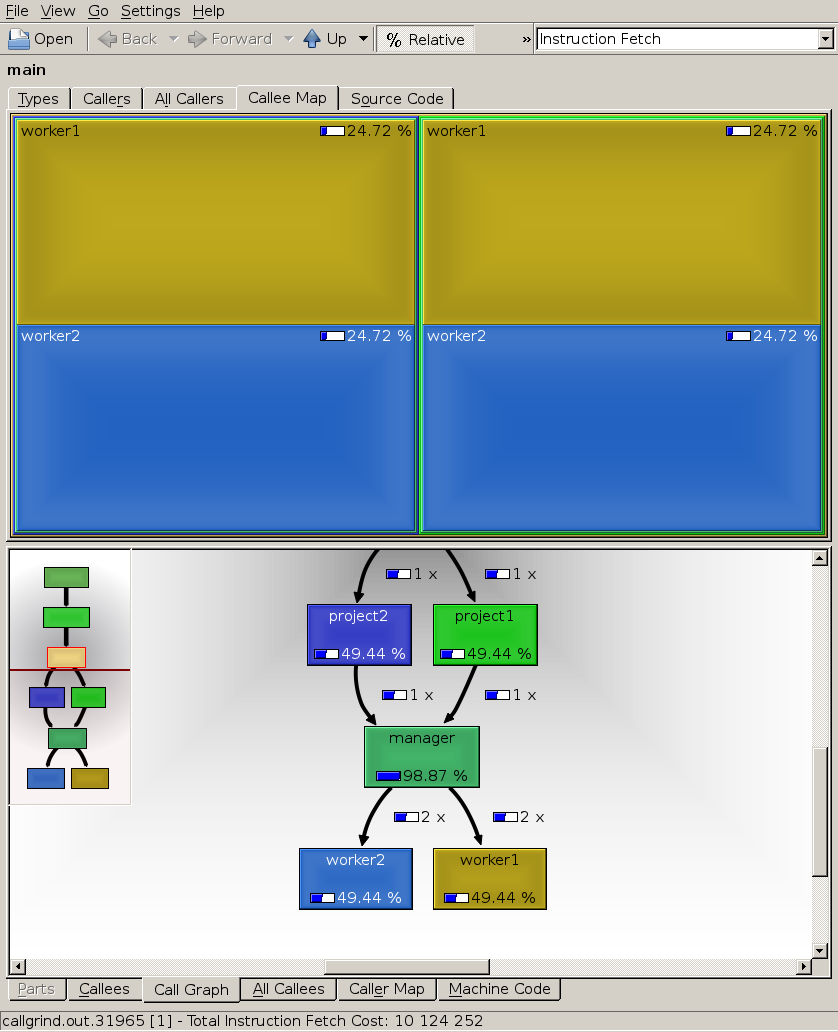
\includegraphics[width=.5\textwidth]{images/kcachegrind2}
  \end{center}
\end{frame}
%%%%%%%%%%%%%%%%%%%%%%%%%%%%%%%%%%%%%%%%%%%%%%%%%%%%%%%%%%%%%%%%%%%%%%%%%%%%%%%%

%%%%%%%%%%%%%%%%%%%%%%%%%%%%%%%%%%%%%%%%%%%%%%%%%%%%%%%%%%%%%%%%%%%%%%%%%%%%%%%%
\begin{frame}
  \frametitle{KCacheGrind Truths}
  \begin{center}
    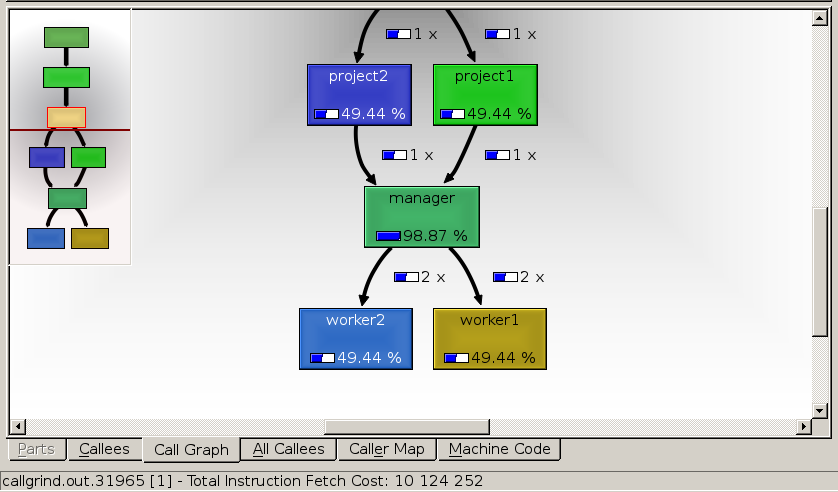
\includegraphics[width=.5\textwidth]{images/kcachegrind2-bottom}
  \end{center}
  
    This is the call graph.\\
    {\tt worker1} and {\tt worker2} do each take about 50\% of time.\\
    So do {\tt project2} and {\tt project1}.\\[1em]
    (gprof would interpolate that too.)
  
\end{frame}
%%%%%%%%%%%%%%%%%%%%%%%%%%%%%%%%%%%%%%%%%%%%%%%%%%%%%%%%%%%%%%%%%%%%%%%%%%%%%%%%

%%%%%%%%%%%%%%%%%%%%%%%%%%%%%%%%%%%%%%%%%%%%%%%%%%%%%%%%%%%%%%%%%%%%%%%%%%%%%%%%
\begin{frame}
  \frametitle{KCacheGrind Lies}
  \begin{center}
    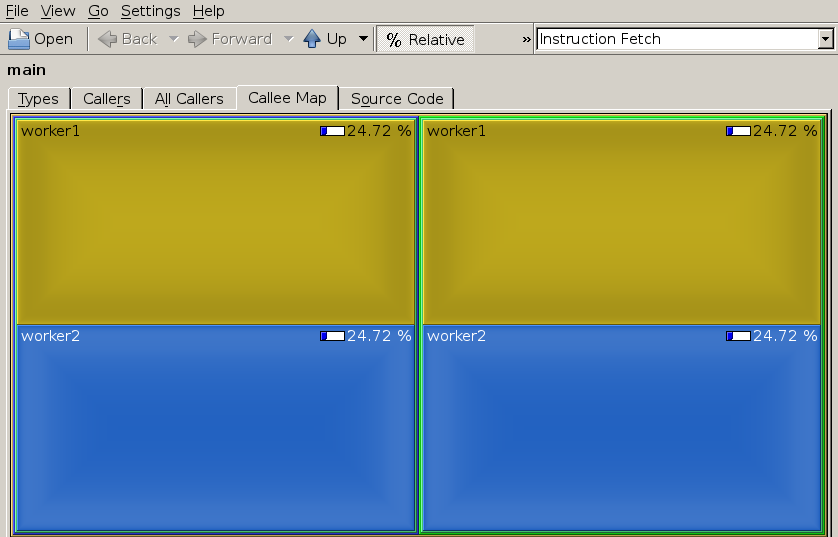
\includegraphics[width=.5\textwidth]{images/kcachegrind2-top}
  \end{center}
  
    KCacheGrind is reporting:
    \begin{itemize}
    \item {\tt worker1} and {\tt worker2} doing \\
      half the work in each project.
    \end{itemize}
    That's not what the code says.
  
\end{frame}
%%%%%%%%%%%%%%%%%%%%%%%%%%%%%%%%%%%%%%%%%%%%%%%%%%%%%%%%%%%%%%%%%%%%%%%%%%%%%%%%

%%%%%%%%%%%%%%%%%%%%%%%%%%%%%%%%%%%%%%%%%%%%%%%%%%%%%%%%%%%%%%%%%%%%%%%%%%%%%%%%
\begin{frame}
  \frametitle{Why KCacheGrind Lies}

  \begin{itemize}
  \item gprof reports time spent in {\tt f()} and {\tt g()},\\
    and how many times {\tt f()} calls {\tt g()}.
  \item callgrind also reports \\
     time spent  in {\tt g()}
     when called from {\tt f()}, \\
     i.e. some calling-context information.\\[1em]
   \item callgrind does \emph{not} report time spent in {\tt g()} \\
     when
     called from {\tt f()} when called from {\tt h()}.\\[1em]
     We don't get the {\tt project1} to {\tt manager} to {\tt worker1} link.\\[1em]
     \item (We have Edges but need Edge-Pairs).
     \end{itemize}
  
\end{frame}
%%%%%%%%%%%%%%%%%%%%%%%%%%%%%%%%%%%%%%%%%%%%%%%%%%%%%%%%%%%%%%%%%%%%%%%%%%%%%%%%

%%%%%%%%%%%%%%%%%%%%%%%%%%%%%%%%%%%%%%%%%%%%%%%%%%%%%%%%%%%%%%%%%%%%%%%%%%%%%%%%
\begin{frame}
  \frametitle{gprof/KCacheGrind summary}
  
    Some results are exact;\\
    some results are sampled;\\
    some results are interpolated.\\[1em]

    If you understand the tool, \\
    you understand where it can go wrong.\\[1em]

    Understand your tools!
  
\end{frame}
%%%%%%%%%%%%%%%%%%%%%%%%%%%%%%%%%%%%%%%%%%%%%%%%%%%%%%%%%%%%%%%%%%%%%%%%%%%%%%%%

\part{Lies from Metrics}

%%%%%%%%%%%%%%%%%%%%%%%%%%%%%%%%%%%%%%%%%%%%%%%%%%%%%%%%%%%%%%%%%%%%%%%%%%%%%%%%
\begin{frame}
  \partpage
\end{frame}
%%%%%%%%%%%%%%%%%%%%%%%%%%%%%%%%%%%%%%%%%%%%%%%%%%%%%%%%%%%%%%%%%%%%%%%%%%%%%%%%

%%%%%%%%%%%%%%%%%%%%%%%%%%%%%%%%%%%%%%%%%%%%%%%%%%%%%%%%%%%%%%%%%%%%%%%%%%%%%%%%
\begin{frame}
  \frametitle{Lying perf counters}
  
  
    While app-specific metrics can lie too,\\
    mostly we'll talk about CPU perf counters.
  



  \begin{center}
    Reference: Paul Khuong,\\
  \tiny
  \url{http://www.pvk.ca/Blog/2014/10/19/performance-optimisation-~-writing-an-essay/}

  \end{center}

\end{frame}
%%%%%%%%%%%%%%%%%%%%%%%%%%%%%%%%%%%%%%%%%%%%%%%%%%%%%%%%%%%%%%%%%%%%%%%%%%%%%%%%

%%%%%%%%%%%%%%%%%%%%%%%%%%%%%%%%%%%%%%%%%%%%%%%%%%%%%%%%%%%%%%%%%%%%%%%%%%%%%%%%
\begin{frame}
  \frametitle{mfence}


    We've talked about {\tt mfence}.\\
    Used in spinlocks, for instance.\\[2em]
    Profiles said: spinlocking didn't take much time.\\
    Empirically: eliminating spinlocks = better than expected!
    
  
  
\end{frame}
%%%%%%%%%%%%%%%%%%%%%%%%%%%%%%%%%%%%%%%%%%%%%%%%%%%%%%%%%%%%%%%%%%%%%%%%%%%%%%%%

%%%%%%%%%%%%%%%%%%%%%%%%%%%%%%%%%%%%%%%%%%%%%%%%%%%%%%%%%%%%%%%%%%%%%%%%%%%%%%%%
\begin{frame}
  \frametitle{Exploring the lie}

  
    Next step: create microbenchmarks.\\[1em]
    Memory accesses to uncached locations,\\
    or computations,\\[1em]
    surrounded by store pairs/mfence/locks.\\[1em]
    Use perf to evaluate impact of mfence vs lock.
  

\end{frame}
%%%%%%%%%%%%%%%%%%%%%%%%%%%%%%%%%%%%%%%%%%%%%%%%%%%%%%%%%%%%%%%%%%%%%%%%%%%%%%%%

%%%%%%%%%%%%%%%%%%%%%%%%%%%%%%%%%%%%%%%%%%%%%%%%%%%%%%%%%%%%%%%%%%%%%%%%%%%%%%%%
\begin{frame}[fragile]
  \frametitle{perf for lock}

    \begin{lstlisting}
$ perf annotate -s cache_misses
[...]
    0.06 :        4006b0:       and    %rdx,%r10
    0.00 :        4006b3:       add    $0x1,%r9
    ;; random (out of last level cache) read
    0.00 :        4006b7:       mov    (%rsi,%r10,8),%rbp
   30.37 :        4006bb:       mov    %rcx,%r10
    ;; foo is cached, to simulate our internal lock
    0.12 :        4006be:       mov    %r9,0x200fbb(%rip)
    0.00 :        4006c5:       shl    $0x17,%r10
    [... Skipping arithmetic with < 1% weight in the profile]
    ;; locked increment of an in-cache "lock" byte
    1.00 :        4006e7:       lock incb 0x200d92(%rip)
   21.57 :        4006ee:       add    $0x1,%rax
    [...]
    ;; random out of cache read
    0.00 :        400704:       xor    (%rsi,%r10,8),%rbp
   21.99 :        400708:       xor    %r9,%r8
    [...]
    ;; locked in-cache decrement
    0.00 :        400729:       lock decb 0x200d50(%rip)
   18.61 :        400730:       add    $0x1,%rax
    [...]
    0.92 :        400755:       jne    4006b0 <cache_misses+0x30>
    \end{lstlisting}


\end{frame}
%%%%%%%%%%%%%%%%%%%%%%%%%%%%%%%%%%%%%%%%%%%%%%%%%%%%%%%%%%%%%%%%%%%%%%%%%%%%%%%%

%%%%%%%%%%%%%%%%%%%%%%%%%%%%%%%%%%%%%%%%%%%%%%%%%%%%%%%%%%%%%%%%%%%%%%%%%%%%%%%%
\begin{frame}
  \frametitle{lock's effects}

  
    Reads take 30 + 22 = 52\% of runtime\\
    Locks take 19 + 21 = 40\%.
  

\end{frame}
%%%%%%%%%%%%%%%%%%%%%%%%%%%%%%%%%%%%%%%%%%%%%%%%%%%%%%%%%%%%%%%%%%%%%%%%%%%%%%%%

%%%%%%%%%%%%%%%%%%%%%%%%%%%%%%%%%%%%%%%%%%%%%%%%%%%%%%%%%%%%%%%%%%%%%%%%%%%%%%%%
\begin{frame}[fragile]
  \frametitle{perf for mfence}

  \begin{lstlisting}
$ perf annotate -s cache_misses
[...]
    0.00 :        4006b0:       and    %rdx,%r10
    0.00 :        4006b3:       add    $0x1,%r9
    ;; random read
    0.00 :        4006b7:       mov    (%rsi,%r10,8),%rbp
   42.04 :        4006bb:       mov    %rcx,%r10
    ;; store to cached memory (lock word)
    0.00 :        4006be:       mov    %r9,0x200fbb(%rip)
    [...]
    0.20 :        4006e7:       mfence 
    5.26 :        4006ea:       add    $0x1,%rax
    [...]
    ;; random read
    0.19 :        400700:       xor    (%rsi,%r10,8),%rbp
   43.13 :        400704:       xor    %r9,%r8
    [...]
    0.00 :        400725:       mfence 
    4.96 :        400728:       add    $0x1,%rax
    0.92 :        40072c:       add    $0x1,%rax
    [...]
    0.36 :        40074d:       jne    4006b0 <cache_misses+0x30>
  \end{lstlisting}

\end{frame}
%%%%%%%%%%%%%%%%%%%%%%%%%%%%%%%%%%%%%%%%%%%%%%%%%%%%%%%%%%%%%%%%%%%%%%%%%%%%%%%%

%%%%%%%%%%%%%%%%%%%%%%%%%%%%%%%%%%%%%%%%%%%%%%%%%%%%%%%%%%%%%%%%%%%%%%%%%%%%%%%%
\begin{frame}
  \frametitle{mfence's effects}

  
    Looks like the reads take 85\% of runtime,\\
    while the mfence takes 15\% of runtime.
  

\end{frame}
%%%%%%%%%%%%%%%%%%%%%%%%%%%%%%%%%%%%%%%%%%%%%%%%%%%%%%%%%%%%%%%%%%%%%%%%%%%%%%%%

%%%%%%%%%%%%%%%%%%%%%%%%%%%%%%%%%%%%%%%%%%%%%%%%%%%%%%%%%%%%%%%%%%%%%%%%%%%%%%%%
\begin{frame}
  \frametitle{Bigger picture}

  
    Must also look at total \# of cycles.\\[1em]
    \begin{tabular}{lr}
    No atomic/fence:& 2.81e9 cycles\\
    lock inc/dec: & 3.66e9 cycles\\
    mfence: & 19.60e9 cycles
    \end{tabular}
~\\[1em]
    That 15\% number is a total lie.
  
  \begin{center}
	
\includegraphics[width=0.3\textwidth]{images/maury.jpg}
\end{center}

\end{frame}
%%%%%%%%%%%%%%%%%%%%%%%%%%%%%%%%%%%%%%%%%%%%%%%%%%%%%%%%%%%%%%%%%%%%%%%%%%%%%%%%

%%%%%%%%%%%%%%%%%%%%%%%%%%%%%%%%%%%%%%%%%%%%%%%%%%%%%%%%%%%%%%%%%%%%%%%%%%%%%%%%
\begin{frame}
  \frametitle{Conclusions}

  
    \begin{itemize}
    \item mfence underestimated;
      \item lock overestimated.
    \end{itemize}
    ~\\
    Why? \\[1em]
    mfence = pipeline flush,\\
    costs attributed to instructions being flushed.\\
  

\end{frame}
%%%%%%%%%%%%%%%%%%%%%%%%%%%%%%%%%%%%%%%%%%%%%%%%%%%%%%%%%%%%%%%%%%%%%%%%%%%%%%%%




\begin{frame}
\frametitle{The Long Tail}

Suppose we have a task that's going to get distributed over multiple computers (like a search). 

If we look at the latency distribution, the problem is mostly that we see a long tail of events. 

When we are doing a computation or search where we need all the results, we can only go as the slowest step.

\end{frame}



\begin{frame}
\frametitle{Grab the Tiger by the Tail}

\begin{center}
	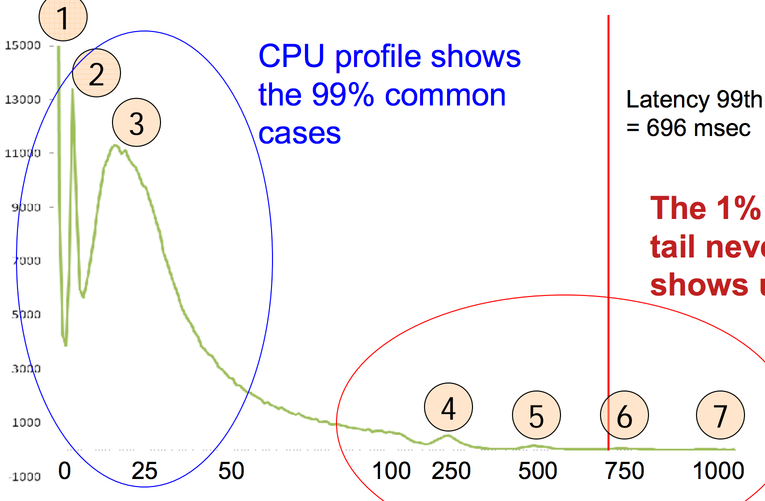
\includegraphics[width=0.85\textwidth]{images/disk_tail.png}
\end{center}

\end{frame}



\begin{frame}
\frametitle{Explaining the Peaks}

\begin{enumerate}
	\item Found in RAM
	\item Disk Cache
	\item Disk
	\item and above... very strange!
\end{enumerate}

\end{frame}



\begin{frame}
\frametitle{Why 250, 500, 750, 1000?}

Answer: CPU throttling!

This was happening on 25\% of disk servers at Google, for an average of half an hour a day!

\end{frame}



\begin{frame}
\frametitle{Faster than a Speeding Bullet}

Another problem with sampling,
this time from Lucene:

\begin{center}
	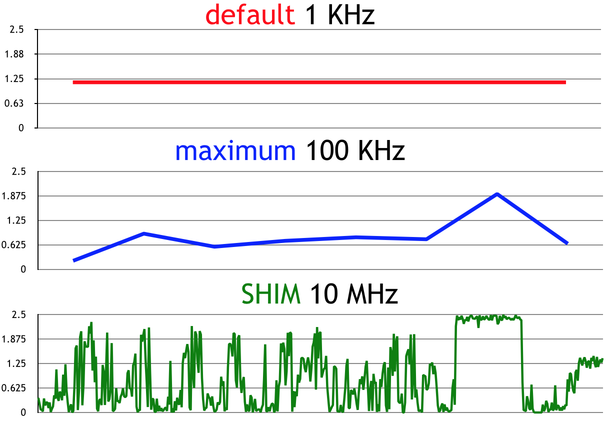
\includegraphics[width=0.7\textwidth]{images/perf-sample.png}
\end{center}

Why is perf limited to 100~KHz?

\end{frame}



\begin{frame}
\frametitle{Processing Interrupts}

Answer: perf samples are done with interrupts (slow). 

If you crank up the rate of interrupts, before long, you are spending all your time handling the interrupts rather than doing useful work.

SHIM gets around this by being more invasive.

This produces a bunch of data which can be dealt with later.

\end{frame}


\end{document}

